\documentclass[12pt]{article}
\usepackage[utf8]{inputenc}

\usepackage{lmodern}

\usepackage{enumitem}
\usepackage[margin=2cm]{geometry}

\usepackage{amsmath, amsfonts, amssymb}
\usepackage{graphicx}
%\usepackage{subfigure}
\usepackage{tikz}
\usepackage{pgfplots}
\usepackage{multicol}

\usepackage{comment}
\usepackage{url}
\usepackage{calc}
\usepackage{subcaption}
\usepackage[indent=0pt]{parskip}
\usepackage{animate}

\usepackage{array}
\usepackage{blkarray,booktabs, bigstrut}
\usepackage{bigints}

\pgfplotsset{compat=1.16}

% MATH commands
\newcommand{\ga}{\left\langle}
\newcommand{\da}{\right\rangle}
\newcommand{\oa}{\left\lbrace}
\newcommand{\fa}{\right\rbrace}
\newcommand{\oc}{\left[}
\newcommand{\fc}{\right]}
\newcommand{\op}{\left(}
\newcommand{\fp}{\right)}

\newcommand{\bi}{\mathbf{i}}
\newcommand{\bj}{\mathbf{j}}
\newcommand{\bk}{\mathbf{k}}
\newcommand{\bF}{\mathbf{F}}

\newcommand{\mR}{\mathbb{R}}

\newcommand{\ra}{\rightarrow}
\newcommand{\Ra}{\Rightarrow}

\newcommand{\sech}{\mathrm{sech}\,}
\newcommand{\csch}{\mathrm{csch}\,}
\newcommand{\curl}{\mathrm{curl}\,}
\newcommand{\dive}{\mathrm{div}\,}

\newcommand{\ve}{\varepsilon}
\newcommand{\spc}{\vspace*{0.5cm}}

\DeclareMathOperator{\Ran}{Ran}
\DeclareMathOperator{\Dom}{Dom}

\newcommand{\exo}[1]{\noindent\textcolor{red}{\fbox{\textbf{Problem {#1}}}\hrulefill}\\\\ }
\newcommand{\qu}[4]{\noindent\textcolor{#4}{\fbox{\textbf{Section {#1} | Problem {#2}}} \hrulefill{{\fbox{\textbf{{#3} Points}}}}\\}}

\newcommand{\semester}{Fall 2023}

\newcommand{\CVup}{%
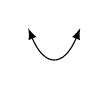
\begin{tikzpicture}
\draw[black, <->, >=latex] (-0.33, 0.5) .. controls (-0.125, 0) and (0.125, 0) .. (0.33, 0.5);
\end{tikzpicture}}

\newcommand{\CVupInc}{%
\begin{tikzpicture}
\draw[black, ->, >=latex] (0,0) .. controls (0.2, 0) and (0.4, 0.2) .. (0.5, 0.5);
\end{tikzpicture}}

\newcommand{\CVupDec}{%
\begin{tikzpicture}[rotate=270]
\draw[black, ->, >=latex] (0,0) .. controls (0.2, 0) and (0.4, 0.2) .. (0.5, 0.5);
\end{tikzpicture}}

\newcommand{\CVdown}{%
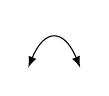
\begin{tikzpicture}
\draw[black, <->, >=latex] (-0.33, -0.5) .. controls (-0.125, 0) and (0.125, 0) .. (0.33, -0.5);
\end{tikzpicture}}

\newcommand{\CVdownInc}{%
\begin{tikzpicture}
\draw[black, ->, >=latex] (-0.5, -0.5) .. controls (-0.5, -0.3) and (-0.5, -0.1) .. (0,0);
\end{tikzpicture}}

\newcommand{\CVdownDec}{%
\begin{tikzpicture}[rotate=-90]
\draw[black, ->, >=latex] (-0.5, -0.5) .. controls (-0.5, -0.3) and (-0.5, -0.1) .. (0,0);
\end{tikzpicture}}

\begin{document}
	\noindent \hrulefill \\
	MATH-244 \semester \hfill Practice Problems Solutions\\
	Section 16.6 \hfill Pierre-Olivier Paris{\'e} \\\vspace*{-1cm}
	
	\noindent\hrulefill
	
	\spc	
	
	\exo{10}
	\vspace*{-0.5cm}
	\begin{enumerate}
	\item[(a)] By definition, $\mathrm{div}\, \vec{F} = P_x + Q_y + R_z = P_x + Q_y$ because $R$ is independent of $z$.
	
	If we look only at the $x$ components of $\vec{F}$, that is $P$, we observe that when $y$ varies, there is no change in $P$ (the first coordinate of the vectors in $\vec{F}$), but when $x$ varies, there is a change in $P$. This change is positive because when $x$ increases, the values of $P$ increasin, this means that $P_x > 0$.
	
	If we look only at the $y$-components of the vectors in $\vec{F}$, that is $Q$, we observe that when $x$ varies, there is no change in $Q$ (the second coordinate of the vectors in $\vec{F}$), but when $y$ varies, there is a change in $Q$. This change is positive because when $y$ increases, the values of $Q$ increase, this means that $Q_y > 0$. 
	
	Thus, overall, we have $P_x + Q_y > 0$, meaning that $\mathrm{div} \vec{F} > 0$.
	
	\item[(b)] The fact that $\vec{F}$ doesn't depend on $z$ implies that $\mathrm{curl} \vec{F} = \left\langle 0 , 0 , Q_x - P_y \right\rangle$. Thus, depending on the sign of $Q_x - P_y$, the vector $\mathrm{curl} \vec{F}$ is orthogonal to the $XY$-plane and points in the direction of the positive $z$-axis if $Q_x - P_y > 0$ and in the direction of the negative $z$-axis if $Q_x - P_y < 0$.
	\end{enumerate}
	
	\spc
	
	\exo{2 (only Q)}
	We have to check if there are $u, v$ such that $\vec{r} (u, v) = \left\langle 2, 3, 3 \right\rangle$.
	
	%For the point $P$, this means we have to solve the three following questions:
	%	\begin{align*}
	%	1 + u - v = 1, \quad u + v^2 = 2, \quad u^2 - v^2 = 1 .
	%	\end{align*}
	%Adding the second equation to the third equation, we obtain the following
	%	\begin{align*}
	%	u + u^2 = 3 \quad \Ra \quad u^2 + u - 3 = 0 .
	%	\end{align*}
	%Using the quadratic formula, we see that the solutions must be
	%	\begin{align*}
	%	u = \frac{-1 \pm \sqrt{1 + 12}}{2} = \frac{-1 \pm \sqrt{13}}{2} .
	%	\end{align*}
	%We only need one value for $u$, say $u = (1 + \sqrt{13})/2$. From the first equation, we see that $u = v$ and so $v = (1 + \sqrt{13})/2$ also. We just found $(u, v)$ such that $\vec{r} (u, v) = \left\langle 1, 2, 1 \right\rangle$ which mean that the point $P$ lies on the surface.
	
	For the point $Q$, this means we have to solve the three following equations:
	\begin{align*}
		1 + u - v = 2, \quad u + v^2 = 3, \quad u^2 - v^2 = 3 .
		\end{align*}
	Adding the second equation to the third equation, we obtain
		\begin{align*}
		u^2 + u = 6 \quad \Ra \quad u^2 + u - 6 = 0 \quad \Ra \quad (u + 3) (u - 2) = 0 .
		\end{align*}
	The solutions are $u = -3$ and $u = 2$. we just need one value, say $u = 2$. From the first equation, we see that $u = v$ and so $v = 3$. We just found $(u, v)$ such that $\vec{r} (u, v) = \left\langle 1, 2, 1 \right\rangle$ which mean that the point $P$ lies on the surface.
	
	\spc
	
	\exo{12}
	Using either the software on the web, or the python script that I provided, you obtain the following images.
	
	\begin{figure}[h]
	\centering
	\begin{subfigure}[b]{0.45\textwidth}
		\centering
		\includegraphics[scale=0.35]{picture1.png}
		\caption{Graph of the surface}
	\end{subfigure}
	\begin{subfigure}[b]{0.45\textwidth}
		\centering
		\includegraphics[scale=0.3]{picture2.png}
		\caption{Latitudes when $u$ is constant}
	\end{subfigure}
	\begin{subfigure}[b]{0.45\textwidth}
		\centering
		\includegraphics[scale=0.3]{picture3.png}
		\caption{Longitudes when $v$ is constant}
	\end{subfigure}
	\begin{subfigure}[b]{0.45\textwidth}
		\centering	
		\includegraphics[scale=0.3]{picture4.png}
		\caption{Grid on the surface}
	\end{subfigure}
	\end{figure}

	This surface is really funny, it looks like a pillow, a really confortable pillow! :)
	
	\spc
	
	\exo{20}
	The parametric equation is 
		\begin{align*}
		\vec{r} (u, v) = \left\langle 0, -1, 5 \right\rangle + u \left\langle 2, 1, 4 \right\rangle + \left\langle -3, 2, 5 \right\rangle = \left\langle 2u - 3v , -1 + u + 2v , 5 + 4u + 5v \right\rangle .
		\end{align*}
		
	\spc
		
	\exo{26}
	The point $(0, 0, 3)$ lies in the plane. The intersection of a plane and a cylinder is a circle in 3D. So the region will be the interior of a circle (but the circle is not parallel to one of the three planes).
	
	An efficient way of solving this problem is to find two orthogonal vector $\vec{a}$ and $\vec{b}$ parallel to the plane such that they belong to the cylinder and then take a linear combinaison $\left\langle 0, 0, 3 \right\rangle + u \vec{a} + v \vec{b}$ where $u^2 + v^2 \leq 1$. 
	
	 A vector parallel to the plane $z = x + 3$ is a vector $\vec{a} =  \left\langle a_1 , a_2 , a_3 \right\rangle$ which is orthogonal to the normal vector of the plane. The normal vector of the plane is $\vec{n} = \left\langle -1, 0, 1 \right\rangle$. We would also like the tip of the vector $\vec{a}$ belongs to the cylinder, so we also require that $a_1^2 + a_2^2 = 1$. We have to solve
	 	\begin{align*}
	 	\vec{a} \cdot \vec{n} &= 0 \\
	 	a_1^2 + a_2^2 &= 1 .
	 	\end{align*}
	This system is explicitly:
		\begin{align*}
		-a_1 + a_3 &= 0 \\
		a_1^2 + a_2^2 &= 1 .
		\end{align*}
	Since $a_2$ is free, we may put $a_2 = 0$ and so $a_1 = \pm 1$. We keep $a_1 = 1$ and from the first equation, we get $a_3 = 1$. Our vector is then $\vec{a} = \left\langle 1 , 0 , 1 \right\rangle$.  
	
	We have to find a vector $\vec{b} = \left\langle b_1 , b_2 , b_3 \right\rangle$ perpendicular to $\vec{a}$ and lying on the cylinder. These conditions give the following system of equations:
		\begin{align*}
		\vec{b} \cdot \vec{a} &= 0 \\
		b_1^2 + b_2^2 &= 1 .
		\end{align*}
	Explicitly, it gives the following system of equations:
		\begin{align*}
		b_1 + b_3 & = 0 \\
		b_1^2 + b_2^2 & = 1 .
		\end{align*}
	A solution to this system is $b_1 = b_3 = 0$ and $b_2 = 1$. So, we obtain $\vec{b} = \left\langle 0, 1, 0 \right\rangle$. 
	
	Now, we can combine the vectors $\vec{a}$ and $\vec{b}$ with the vector $\left\langle 0, 0, 3 \right\rangle$ (the points on the plane), to obtain
		\begin{align*}
		\vec{r} (u, v) = \left\langle 0 , 0, 3 \right\rangle + u \vec{a} + v \vec{b} .
		\end{align*}
	Since $u^2 + v^2 \leq 1$, we can use polar coordinates $u = \rho\cos \theta$ and $v = \rho \sin \theta$ with $0 \leq \rho \leq 1$ and $0 \leq \theta \leq 2\pi$. Thus, we get, after collecting all the terms together, the following parametrization of the surface:
		\begin{align*}
		\vec{r} (u, v) = \left\langle \rho \cos \theta , \rho \sin \theta , 3 + \rho \cos \theta \right\rangle .
		\end{align*}
		
	There is another solution, which is even simpler. We want the portion of the plane inside the cylinder $x^2 + y^2 = 1$. This means that we want the region $x^2 + y^2 \leq 1$. We can parametrized this region in polar coordinates by setting $x = \rho \cos \theta$ and $y = \rho \sin \theta$ with $0 \leq \rho \leq 1$ and $0 \leq \theta \leq 2\pi$. We can then replace the value of $x$ inside the expression of $z$ to get $z = 3 + \rho \cos \theta$. We then get
		\begin{align*}
		\vec{r} (\rho , \theta ) = \left\langle \rho \cos \theta , \rho \sin \theta , 3 + \rho \cos \theta \right\rangle .
		\end{align*}
	
	\begin{figure}
		\centering
		\includegraphics[scale=0.6]{picture5.png}
		\caption{Surface obtained from the parametrization}
	\end{figure}
	
	\spc
	
	\exo{38}
	We have $\vec{r}_u = \left\langle -2u , 0, -1 \right\rangle$ and $\vec{r}_v = \left\langle -2v , -1 , 0 \right\rangle$. 
	
	We have to find the point $(u_0, v_0)$ such that $\vec{r}(u_0, v_0) = (-1, -1, -1)$. Analyzing the second and third components, we see that $v = 1$ and $u = 1$. Thus, the tangent vectors at $(-1, -1, -1)$ are
		\begin{align*}
		\vec{r}_u (1, 1) = \left\langle -2, 0, -1 \right\rangle \quad \text{ and } \quad \vec{r}_v (1, 1) = \left\langle -2, -1, 0 \right\rangle .
		\end{align*}
	Thus, the parametric equation of the tangent plane is
		\begin{align*}
		\vec{r}_{\Pi} (u, v) = \left\langle -1, -1, -1 \right\rangle + u \vec{r}_u (1, 1) + v \vec{r}_v (1, 1) = \left\langle -1 - 2u -2v , -1 - v , -1 - u \right\rangle 
		\end{align*}
	where $\Pi$ is the name of the plane (the symbol $\Pi$ is the capital $p$ in greek).
	
	Using python, we obtain the following picture of the tangent plane and the surface.
		\begin{figure}[h]
		\centering
		\includegraphics[scale=0.5]{picture6.png}
		\caption{Graph of the surface and its tangent vector}
		\end{figure}
	
\end{document}